\documentclass{book}
\usepackage[a4paper,top=2.5cm,bottom=2.5cm,left=2.5cm,right=2.5cm]{geometry}
\usepackage{makeidx}
\usepackage{natbib}
\usepackage{graphicx}
\usepackage{multicol}
\usepackage{float}
\usepackage{listings}
\usepackage{color}
\usepackage{ifthen}
\usepackage[table]{xcolor}
\usepackage{textcomp}
\usepackage{alltt}
\usepackage{ifpdf}
\ifpdf
\usepackage[pdftex,
            pagebackref=true,
            colorlinks=true,
            linkcolor=blue,
            unicode
           ]{hyperref}
\else
\usepackage[ps2pdf,
            pagebackref=true,
            colorlinks=true,
            linkcolor=blue,
            unicode
           ]{hyperref}
\usepackage{pspicture}
\fi
\usepackage[utf8]{inputenc}
\usepackage{mathptmx}
\usepackage[scaled=.90]{helvet}
\usepackage{courier}
\usepackage{sectsty}
\usepackage{amssymb}
\usepackage[titles]{tocloft}
\usepackage{doxygen}
\lstset{language=C++,inputencoding=utf8,basicstyle=\footnotesize,breaklines=true,breakatwhitespace=true,tabsize=4,numbers=left }
\makeindex
\setcounter{tocdepth}{3}
\renewcommand{\footrulewidth}{0.4pt}
\renewcommand{\familydefault}{\sfdefault}
\hfuzz=15pt
\setlength{\emergencystretch}{15pt}
\hbadness=750
\tolerance=750
\begin{document}
\hypersetup{pageanchor=false,citecolor=blue}
\begin{titlepage}
\vspace*{7cm}
\begin{center}
{\Large Swt\-Lib\-No\-S\-Q\-L }\\
\vspace*{1cm}
{\large Generated by Doxygen 1.8.3.1}\\
\vspace*{0.5cm}
{\small Sat Mar 2 2013 22:52:55}\\
\end{center}
\end{titlepage}
\clearemptydoublepage
\pagenumbering{roman}
\tableofcontents
\clearemptydoublepage
\pagenumbering{arabic}
\hypersetup{pageanchor=true,citecolor=blue}
\chapter{Namespace Index}
\section{Namespace List}
Here is a list of all documented namespaces with brief descriptions\-:\begin{DoxyCompactList}
\item\contentsline{section}{\hyperlink{namespace_swt_lib}{Swt\-Lib} }{\pageref{namespace_swt_lib}}{}
\end{DoxyCompactList}

\chapter{Hierarchical Index}
\section{Class Hierarchy}
This inheritance list is sorted roughly, but not completely, alphabetically\-:\begin{DoxyCompactList}
\item \contentsline{section}{Swt\-Lib.\-No\-S\-Q\-L\-Account}{\pageref{class_swt_lib_1_1_no_s_q_l_account}}{}
\item \contentsline{section}{Swt\-Lib.\-No\-S\-Q\-L\-Condition}{\pageref{interface_swt_lib_1_1_no_s_q_l_condition}}{}
\begin{DoxyCompactList}
\item \contentsline{section}{Swt\-Lib.\-No\-S\-Q\-L\-Condition$<$ T $>$}{\pageref{class_swt_lib_1_1_no_s_q_l_condition_3_01_t_01_4}}{}
\end{DoxyCompactList}
\item \contentsline{section}{Swt\-Lib.\-No\-S\-Q\-L\-Database}{\pageref{class_swt_lib_1_1_no_s_q_l_database}}{}
\item \contentsline{section}{Swt\-Lib.\-No\-S\-Q\-L\-Filter}{\pageref{class_swt_lib_1_1_no_s_q_l_filter}}{}
\item \contentsline{section}{Swt\-Lib.\-No\-S\-Q\-L\-Table}{\pageref{interface_swt_lib_1_1_no_s_q_l_table}}{}
\item Table\-Entity\begin{DoxyCompactList}
\item \contentsline{section}{Swt\-Lib.\-No\-S\-Q\-L\-Table\-Entity}{\pageref{class_swt_lib_1_1_no_s_q_l_table_entity}}{}
\end{DoxyCompactList}
\end{DoxyCompactList}

\chapter{Class Index}
\section{Class List}
Here are the classes, structs, unions and interfaces with brief descriptions\-:\begin{DoxyCompactList}
\item\contentsline{section}{\hyperlink{class_swt_lib_1_1_no_s_q_l_account}{Swt\-Lib.\-No\-S\-Q\-L\-Account} }{\pageref{class_swt_lib_1_1_no_s_q_l_account}}{}
\item\contentsline{section}{\hyperlink{interface_swt_lib_1_1_no_s_q_l_condition}{Swt\-Lib.\-No\-S\-Q\-L\-Condition} }{\pageref{interface_swt_lib_1_1_no_s_q_l_condition}}{}
\item\contentsline{section}{\hyperlink{class_swt_lib_1_1_no_s_q_l_condition_3_01_t_01_4}{Swt\-Lib.\-No\-S\-Q\-L\-Condition$<$ T $>$} }{\pageref{class_swt_lib_1_1_no_s_q_l_condition_3_01_t_01_4}}{}
\item\contentsline{section}{\hyperlink{class_swt_lib_1_1_no_s_q_l_database}{Swt\-Lib.\-No\-S\-Q\-L\-Database} }{\pageref{class_swt_lib_1_1_no_s_q_l_database}}{}
\item\contentsline{section}{\hyperlink{class_swt_lib_1_1_no_s_q_l_filter}{Swt\-Lib.\-No\-S\-Q\-L\-Filter} \\*Filter is more limited than regular boolean expressions. Motivation to use this limited design is because Amazon uses it and is the weakest link. Other robust and flexible models will require commitment in the design/implementation artifact. If design and implementation plan are clear and easy to execute, I will go forward with the plan. }{\pageref{class_swt_lib_1_1_no_s_q_l_filter}}{}
\item\contentsline{section}{\hyperlink{interface_swt_lib_1_1_no_s_q_l_table}{Swt\-Lib.\-No\-S\-Q\-L\-Table} }{\pageref{interface_swt_lib_1_1_no_s_q_l_table}}{}
\item\contentsline{section}{\hyperlink{class_swt_lib_1_1_no_s_q_l_table_entity}{Swt\-Lib.\-No\-S\-Q\-L\-Table\-Entity} \\*Required inheritance to store class onto No\-S\-Q\-L database using this library. }{\pageref{class_swt_lib_1_1_no_s_q_l_table_entity}}{}
\end{DoxyCompactList}

\chapter{Namespace Documentation}
\hypertarget{namespace_swt_lib}{\section{Package Swt\-Lib}
\label{namespace_swt_lib}\index{Swt\-Lib@{Swt\-Lib}}
}
\subsection*{Classes}
\begin{DoxyCompactItemize}
\item 
class \hyperlink{class_swt_lib_1_1_no_s_q_l_account}{No\-S\-Q\-L\-Account}
\item 
class {\bfseries No\-S\-Q\-L\-Comparison}
\item 
interface \hyperlink{interface_swt_lib_1_1_no_s_q_l_condition}{No\-S\-Q\-L\-Condition}
\item 
class \hyperlink{class_swt_lib_1_1_no_s_q_l_condition_3_01_t_01_4}{No\-S\-Q\-L\-Condition$<$ T $>$}
\item 
class \hyperlink{class_swt_lib_1_1_no_s_q_l_database}{No\-S\-Q\-L\-Database}
\item 
class \hyperlink{class_swt_lib_1_1_no_s_q_l_filter}{No\-S\-Q\-L\-Filter}
\begin{DoxyCompactList}\small\item\em Filter is more limited than regular boolean expressions. Motivation to use this limited design is because Amazon uses it and is the weakest link. Other robust and flexible models will require commitment in the design/implementation artifact. If design and implementation plan are clear and easy to execute, I will go forward with the plan. \end{DoxyCompactList}\item 
interface \hyperlink{interface_swt_lib_1_1_no_s_q_l_table}{No\-S\-Q\-L\-Table}
\item 
class \hyperlink{class_swt_lib_1_1_no_s_q_l_table_entity}{No\-S\-Q\-L\-Table\-Entity}
\begin{DoxyCompactList}\small\item\em Classes that need to be stored in the No\-S\-Q\-L Database must implement this class.  Hi \end{DoxyCompactList}\end{DoxyCompactItemize}

\chapter{Class Documentation}
\hypertarget{class_swt_lib_1_1_no_s_q_l_account}{\section{Swt\-Lib.\-No\-S\-Q\-L\-Account Class Reference}
\label{class_swt_lib_1_1_no_s_q_l_account}\index{Swt\-Lib.\-No\-S\-Q\-L\-Account@{Swt\-Lib.\-No\-S\-Q\-L\-Account}}
}
\subsection*{Properties}
\begin{DoxyCompactItemize}
\item 
\hypertarget{class_swt_lib_1_1_no_s_q_l_account_a4e29bf49b2096d0c31dc492907d472b2}{Cloud\-Storage\-Account {\bfseries Azure\-Account}\hspace{0.3cm}{\ttfamily  \mbox{[}get\mbox{]}}}\label{class_swt_lib_1_1_no_s_q_l_account_a4e29bf49b2096d0c31dc492907d472b2}

\end{DoxyCompactItemize}


The documentation for this class was generated from the following file\-:\begin{DoxyCompactItemize}
\item 
No\-S\-Q\-L\-Account.\-cs\end{DoxyCompactItemize}

\hypertarget{interface_swt_lib_1_1_no_s_q_l_condition}{\section{Swt\-Lib.\-No\-S\-Q\-L\-Condition Interface Reference}
\label{interface_swt_lib_1_1_no_s_q_l_condition}\index{Swt\-Lib.\-No\-S\-Q\-L\-Condition@{Swt\-Lib.\-No\-S\-Q\-L\-Condition}}
}
Inheritance diagram for Swt\-Lib.\-No\-S\-Q\-L\-Condition\-:\begin{figure}[H]
\begin{center}
\leavevmode
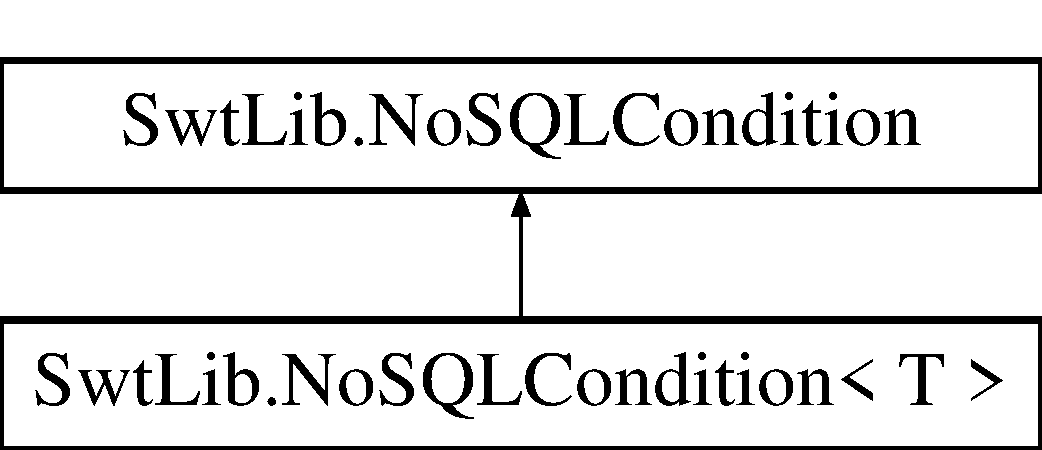
\includegraphics[height=2.000000cm]{interface_swt_lib_1_1_no_s_q_l_condition}
\end{center}
\end{figure}
\subsection*{Properties}
\begin{DoxyCompactItemize}
\item 
\hypertarget{interface_swt_lib_1_1_no_s_q_l_condition_a2967e236c0a99ce54c11febe46d3b05a}{string {\bfseries Variable\-Name}\hspace{0.3cm}{\ttfamily  \mbox{[}get\mbox{]}}}\label{interface_swt_lib_1_1_no_s_q_l_condition_a2967e236c0a99ce54c11febe46d3b05a}

\item 
\hypertarget{interface_swt_lib_1_1_no_s_q_l_condition_a7d1a71fc8c5d277aca90cac92c37408a}{No\-S\-Q\-L\-Comparison.\-Operator {\bfseries Comparison\-Operator}\hspace{0.3cm}{\ttfamily  \mbox{[}get\mbox{]}}}\label{interface_swt_lib_1_1_no_s_q_l_condition_a7d1a71fc8c5d277aca90cac92c37408a}

\item 
\hypertarget{interface_swt_lib_1_1_no_s_q_l_condition_acdcc93815218d406524db265d82fb74e}{dynamic {\bfseries Value}\hspace{0.3cm}{\ttfamily  \mbox{[}get\mbox{]}}}\label{interface_swt_lib_1_1_no_s_q_l_condition_acdcc93815218d406524db265d82fb74e}

\end{DoxyCompactItemize}


The documentation for this interface was generated from the following file\-:\begin{DoxyCompactItemize}
\item 
No\-S\-Q\-L\-Condition.\-cs\end{DoxyCompactItemize}

\hypertarget{class_swt_lib_1_1_no_s_q_l_condition_3_01_t_01_4}{\section{Swt\-Lib.\-No\-S\-Q\-L\-Condition$<$ T $>$ Class Template Reference}
\label{class_swt_lib_1_1_no_s_q_l_condition_3_01_t_01_4}\index{Swt\-Lib.\-No\-S\-Q\-L\-Condition$<$ T $>$@{Swt\-Lib.\-No\-S\-Q\-L\-Condition$<$ T $>$}}
}
Inheritance diagram for Swt\-Lib.\-No\-S\-Q\-L\-Condition$<$ T $>$\-:\begin{figure}[H]
\begin{center}
\leavevmode
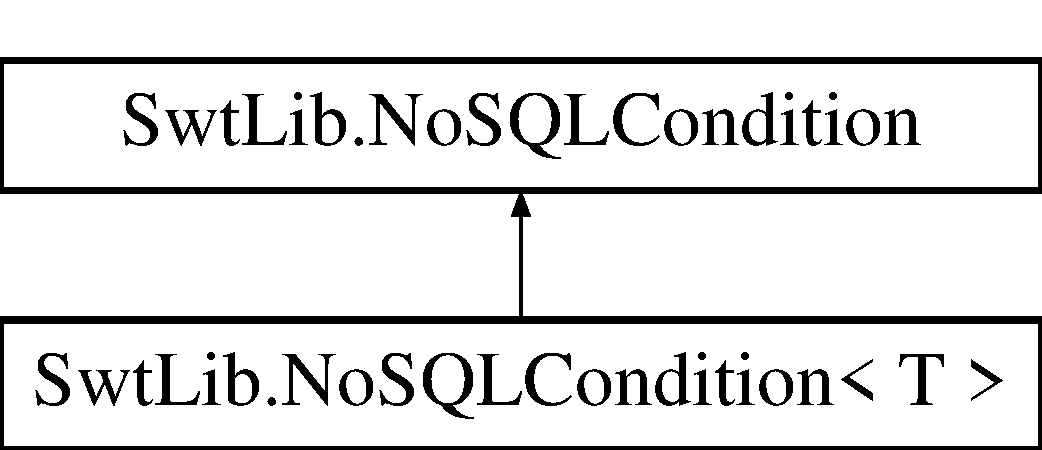
\includegraphics[height=2.000000cm]{class_swt_lib_1_1_no_s_q_l_condition_3_01_t_01_4}
\end{center}
\end{figure}
\subsection*{Public Member Functions}
\begin{DoxyCompactItemize}
\item 
\hypertarget{class_swt_lib_1_1_no_s_q_l_condition_3_01_t_01_4_ab8d2f23ea2009864bb8a973f4d7d0503}{{\bfseries No\-S\-Q\-L\-Condition} (string variable\-Name, No\-S\-Q\-L\-Comparison.\-Operator comparison\-Operator, T value)}\label{class_swt_lib_1_1_no_s_q_l_condition_3_01_t_01_4_ab8d2f23ea2009864bb8a973f4d7d0503}

\end{DoxyCompactItemize}
\subsection*{Properties}
\begin{DoxyCompactItemize}
\item 
\hypertarget{class_swt_lib_1_1_no_s_q_l_condition_3_01_t_01_4_a2fb2ac05d4c8ebfe22e44779b720221c}{string {\bfseries Variable\-Name}\hspace{0.3cm}{\ttfamily  \mbox{[}get\mbox{]}}}\label{class_swt_lib_1_1_no_s_q_l_condition_3_01_t_01_4_a2fb2ac05d4c8ebfe22e44779b720221c}

\item 
\hypertarget{class_swt_lib_1_1_no_s_q_l_condition_3_01_t_01_4_a7b42a24d3ded412e244efb784ad5f81e}{No\-S\-Q\-L\-Comparison.\-Operator {\bfseries Comparison\-Operator}\hspace{0.3cm}{\ttfamily  \mbox{[}get\mbox{]}}}\label{class_swt_lib_1_1_no_s_q_l_condition_3_01_t_01_4_a7b42a24d3ded412e244efb784ad5f81e}

\item 
\hypertarget{class_swt_lib_1_1_no_s_q_l_condition_3_01_t_01_4_ae54344945a9c5aeb1043fb6e4f623ece}{T {\bfseries Value}\hspace{0.3cm}{\ttfamily  \mbox{[}get, set\mbox{]}}}\label{class_swt_lib_1_1_no_s_q_l_condition_3_01_t_01_4_ae54344945a9c5aeb1043fb6e4f623ece}

\end{DoxyCompactItemize}


The documentation for this class was generated from the following file\-:\begin{DoxyCompactItemize}
\item 
No\-S\-Q\-L\-Condition.\-cs\end{DoxyCompactItemize}

\hypertarget{class_swt_lib_1_1_no_s_q_l_database}{\section{Swt\-Lib.\-No\-S\-Q\-L\-Database Class Reference}
\label{class_swt_lib_1_1_no_s_q_l_database}\index{Swt\-Lib.\-No\-S\-Q\-L\-Database@{Swt\-Lib.\-No\-S\-Q\-L\-Database}}
}
\subsection*{Public Member Functions}
\begin{DoxyCompactItemize}
\item 
\hypertarget{class_swt_lib_1_1_no_s_q_l_database_a2da613fe1a8427bd2ffc02ebc01c0f60}{abstract \hyperlink{interface_swt_lib_1_1_no_s_q_l_table}{No\-S\-Q\-L\-Table} {\bfseries Create\-Table} (string table\-Name)}\label{class_swt_lib_1_1_no_s_q_l_database_a2da613fe1a8427bd2ffc02ebc01c0f60}

\item 
\hypertarget{class_swt_lib_1_1_no_s_q_l_database_acce068a352112abaa2aabe3da060b19a}{abstract \hyperlink{interface_swt_lib_1_1_no_s_q_l_table}{No\-S\-Q\-L\-Table} {\bfseries Get\-Table} (string table\-Name)}\label{class_swt_lib_1_1_no_s_q_l_database_acce068a352112abaa2aabe3da060b19a}

\item 
\hypertarget{class_swt_lib_1_1_no_s_q_l_database_ab2e777e1f340fb0babe63924cd398d41}{abstract I\-Enumerable$<$ \hyperlink{interface_swt_lib_1_1_no_s_q_l_table}{No\-S\-Q\-L\-Table} $>$ {\bfseries List\-Tables} ()}\label{class_swt_lib_1_1_no_s_q_l_database_ab2e777e1f340fb0babe63924cd398d41}

\end{DoxyCompactItemize}
\subsection*{Static Public Member Functions}
\begin{DoxyCompactItemize}
\item 
\hypertarget{class_swt_lib_1_1_no_s_q_l_database_ae0b7ce581c34a475062af6289293ce0e}{static \hyperlink{class_swt_lib_1_1_no_s_q_l_database}{No\-S\-Q\-L\-Database} {\bfseries Connect} (Microsoft.\-Windows\-Azure.\-Storage.\-Cloud\-Storage\-Account account)}\label{class_swt_lib_1_1_no_s_q_l_database_ae0b7ce581c34a475062af6289293ce0e}

\end{DoxyCompactItemize}


The documentation for this class was generated from the following file\-:\begin{DoxyCompactItemize}
\item 
No\-S\-Q\-L\-Database.\-cs\end{DoxyCompactItemize}

\hypertarget{class_swt_lib_1_1_no_s_q_l_filter}{\section{Swt\-Lib.\-No\-S\-Q\-L\-Filter Class Reference}
\label{class_swt_lib_1_1_no_s_q_l_filter}\index{Swt\-Lib.\-No\-S\-Q\-L\-Filter@{Swt\-Lib.\-No\-S\-Q\-L\-Filter}}
}


Filter is more limited than regular boolean expressions. Motivation to use this limited design is because Amazon uses it and is the weakest link. Other robust and flexible models will require commitment in the design/implementation artifact. If design and implementation plan are clear and easy to execute, I will go forward with the plan.  




\subsection{Detailed Description}
Filter is more limited than regular boolean expressions. Motivation to use this limited design is because Amazon uses it and is the weakest link. Other robust and flexible models will require commitment in the design/implementation artifact. If design and implementation plan are clear and easy to execute, I will go forward with the plan. 



The documentation for this class was generated from the following file\-:\begin{DoxyCompactItemize}
\item 
No\-S\-Q\-L\-Filter.\-cs\end{DoxyCompactItemize}

\hypertarget{interface_swt_lib_1_1_no_s_q_l_table}{\section{Swt\-Lib.\-No\-S\-Q\-L\-Table Interface Reference}
\label{interface_swt_lib_1_1_no_s_q_l_table}\index{Swt\-Lib.\-No\-S\-Q\-L\-Table@{Swt\-Lib.\-No\-S\-Q\-L\-Table}}
}
\subsection*{Public Member Functions}
\begin{DoxyCompactItemize}
\item 
\hypertarget{interface_swt_lib_1_1_no_s_q_l_table_a9b42e3a43065b3231454c33c90280caf}{void {\bfseries Drop} ()}\label{interface_swt_lib_1_1_no_s_q_l_table_a9b42e3a43065b3231454c33c90280caf}

\item 
\hypertarget{interface_swt_lib_1_1_no_s_q_l_table_a6f49d096b6f92580a3dbbf6a368fe4ba}{void {\bfseries Insert} (\hyperlink{class_swt_lib_1_1_no_s_q_l_table_entity}{No\-S\-Q\-L\-Table\-Entity} entity)}\label{interface_swt_lib_1_1_no_s_q_l_table_a6f49d096b6f92580a3dbbf6a368fe4ba}

\item 
\hypertarget{interface_swt_lib_1_1_no_s_q_l_table_a172cb998544a42ca9379d492ab54ceba}{void {\bfseries Insert$<$ T $>$} (\hyperlink{class_swt_lib_1_1_no_s_q_l_table_entity}{No\-S\-Q\-L\-Table\-Entity} entity)}\label{interface_swt_lib_1_1_no_s_q_l_table_a172cb998544a42ca9379d492ab54ceba}

\item 
T \hyperlink{interface_swt_lib_1_1_no_s_q_l_table_a5cc749a886e8f0d7b1023f7a75f713bb}{Get$<$ T $>$} (string partition\-Key, string row\-Key)
\begin{DoxyCompactList}\small\item\em Fetches data from the No\-S\-Q\-L table. \end{DoxyCompactList}\item 
\hypertarget{interface_swt_lib_1_1_no_s_q_l_table_aa04b469df6c164ec2bed3ea86ec37438}{void {\bfseries Delete} (\hyperlink{class_swt_lib_1_1_no_s_q_l_table_entity}{No\-S\-Q\-L\-Table\-Entity} entity)}\label{interface_swt_lib_1_1_no_s_q_l_table_aa04b469df6c164ec2bed3ea86ec37438}

\end{DoxyCompactItemize}


\subsection{Member Function Documentation}
\hypertarget{interface_swt_lib_1_1_no_s_q_l_table_a5cc749a886e8f0d7b1023f7a75f713bb}{\index{Swt\-Lib\-::\-No\-S\-Q\-L\-Table@{Swt\-Lib\-::\-No\-S\-Q\-L\-Table}!Get$<$ T $>$@{Get$<$ T $>$}}
\index{Get$<$ T $>$@{Get$<$ T $>$}!SwtLib::NoSQLTable@{Swt\-Lib\-::\-No\-S\-Q\-L\-Table}}
\subsubsection[{Get$<$ T $>$}]{\setlength{\rightskip}{0pt plus 5cm}T Swt\-Lib.\-No\-S\-Q\-L\-Table.\-Get$<$ T $>$ (
\begin{DoxyParamCaption}
\item[{string}]{partition\-Key, }
\item[{string}]{row\-Key}
\end{DoxyParamCaption}
)}}\label{interface_swt_lib_1_1_no_s_q_l_table_a5cc749a886e8f0d7b1023f7a75f713bb}


Fetches data from the No\-S\-Q\-L table. 


\begin{DoxyTemplParams}{Template Parameters}
{\em T} & Return type.\\
\hline
\end{DoxyTemplParams}

\begin{DoxyParams}{Parameters}
{\em partition\-Key} & Partition key.\\
\hline
{\em row\-Key} & Row key.\\
\hline
\end{DoxyParams}
\begin{DoxyReturn}{Returns}
Returns data as T if data is found. Otherwise, returns null.
\end{DoxyReturn}
\begin{Desc}
\item[Type Constraints]\begin{description}
\item[{\em T} : {\em No\-S\-Q\-L\-Table\-Entity}]\end{description}
\end{Desc}


The documentation for this interface was generated from the following file\-:\begin{DoxyCompactItemize}
\item 
No\-S\-Q\-L\-Table.\-cs\end{DoxyCompactItemize}

\hypertarget{class_swt_lib_1_1_no_s_q_l_table_entity}{\section{Swt\-Lib.\-No\-S\-Q\-L\-Table\-Entity Class Reference}
\label{class_swt_lib_1_1_no_s_q_l_table_entity}\index{Swt\-Lib.\-No\-S\-Q\-L\-Table\-Entity@{Swt\-Lib.\-No\-S\-Q\-L\-Table\-Entity}}
}


Classes that need to be stored in the No\-S\-Q\-L Database must implement this class.  Hi  


Inheritance diagram for Swt\-Lib.\-No\-S\-Q\-L\-Table\-Entity\-:\begin{figure}[H]
\begin{center}
\leavevmode
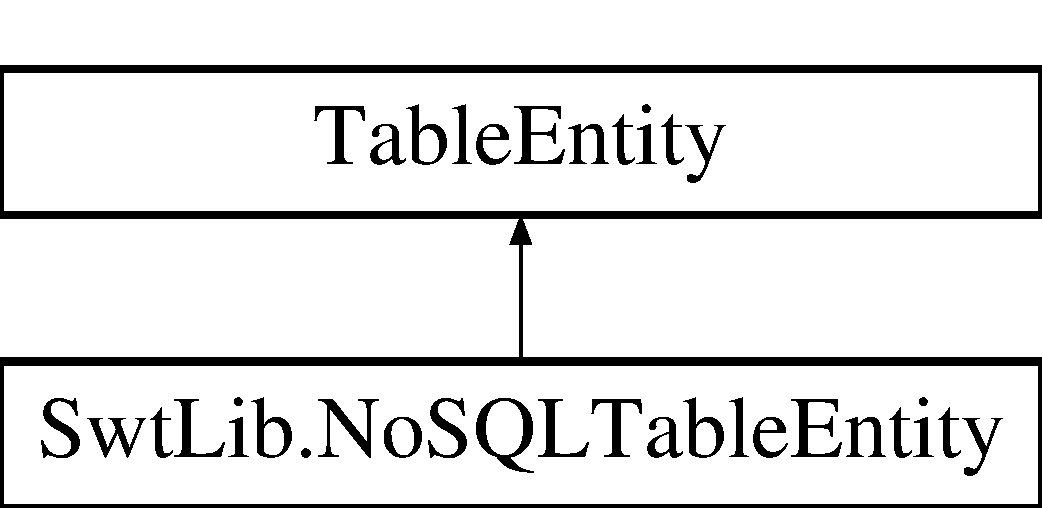
\includegraphics[height=2.000000cm]{class_swt_lib_1_1_no_s_q_l_table_entity}
\end{center}
\end{figure}


\subsection{Detailed Description}
Classes that need to be stored in the No\-S\-Q\-L Database must implement this class.  Hi 



The documentation for this class was generated from the following file\-:\begin{DoxyCompactItemize}
\item 
No\-S\-Q\-L\-Table\-Entity.\-cs\end{DoxyCompactItemize}

\addcontentsline{toc}{part}{Index}
\printindex
\end{document}
